\chapter{Path planning with respect to the end effector}

As of now, we have a fast inverse kinematics algorithm, which allows us to compute joint positions, given the \textit{end effector} position of the manipulator. If we can find a suitable path for the \textit{end effector} to follow, we can discretize it into small steps and use our extension of FABRIK to compute incremental changes along the path for the rest of the manipulator.

Although we have a myriad of algorithms to deal with the 3-dimensional path planning problem, the task is not as simple as our initial example of a robot that can move in any direction; we need to find paths that can be followed with the remainder of the manipulator.

This chapter goes through the process of designing such an algorithm for the task at hand.

\section{Grid based approach}

Recall that one of the successfull ways of applying this technique has been mentioned in~\cite{rrt_fabrik}, where the authors expand a RRT and compute FABRIK at every node. However, our extended FABRIK is too slow to compute for every point in the workspace; hence, we want to limit the amount of times we run the algorithm to lower hundreds.

Therefore, we want to find paths that lead to a solution with a high probability, and only compute FABRIK on points on this path. In case FABRIK fails on this path, for instance due to the manipulator being too short to get around an obstacle, we want to fall back and look for a different path.

Out of the three basic approaches, our go-to are the shortest path in a graph algorithms. As mentioned earlier, gradient based methods are not helpful due to the local minima problem and only generating a single possible path. Similarly, one of the weaknesses of the RRT algorithm is that it only finds a single path, and trying to generate edges between all possible nodes to find multiple paths would be computationally infeasible.

As a baseline for discretization of space, a grid based approach was tested out. This is not optimal for multiple reasons, but it is implementationally simple, allows us to analyze the procedure, and explore further extensions. Note that while the original Djikstra's algorithm works with weighted edges, in this case, we are assigning weights to vertices. Any edge that leads to a given vertex is treated as if it has the weight of the vertex during the shortest path algorithm.

Points on the grid were spaced out at half the size of a single joint, striking a balance between not generating too many points and making the shortest path algorithm too slow, and still being able to explore \textit{most} viable paths\footnote{This claim no longer holds if we consider many tiny obstacles, but the assumption that static objects are of comparable size to the joints of the manipulator is fairly reasonable. Spacing at half the joints' size means that if the manipulator fits in a space between obstacles, it will often be found.}.

The advantage of this representation is that we can weigh the points on the grid to influence which paths will be evaluated as optimal. We borrow the idea from the Artificial Potential Field algorithms, and give more weight to areas that surround an obstacle.

Points on the grid that are occupied by an obstacle are assigned an infinite weight, clearly no path can lead through them. In the area surrounding each obstacle, the weight will be high. Generally, we want the algorithm to choose paths further from obstacles, if possible. This follows the reasoning that we want to accomodate for the rest of the manipulator. If the path for the \textit{end effector} leads closely around obstacles, the chance that the remaining joints of the manipulator will fit is also lowered. However, while expensive, we want the paths close to obstacles to be evaluated as viable, since there may not be other options.

Each obstacle affects the surrounding area and raises the surrounding points on the grid based on how far they are. The total effect of obstacles is summed up; as a result, points between multiple obstacles are given a very high cost. A high cost between clusters of obstacles leads to the desired effect of preferring safer paths that avoid them altogether, though the path itself may be longer.

\begin{figure}
    \centering
    \begin{subfigure}{.3\textwidth}
      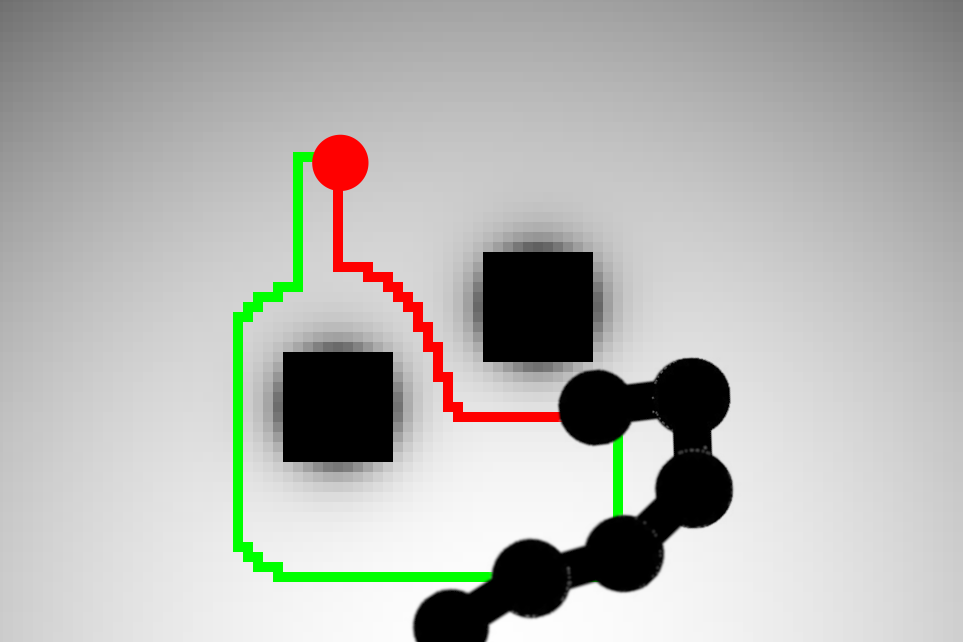
\includegraphics[width=0.99\textwidth]{manipulator_initial.png}
      \caption{Initial position of the manipulator, a target, and the first 2 paths found by the algorithm.}
    \end{subfigure}
    \begin{subfigure}{0.3\textwidth}
      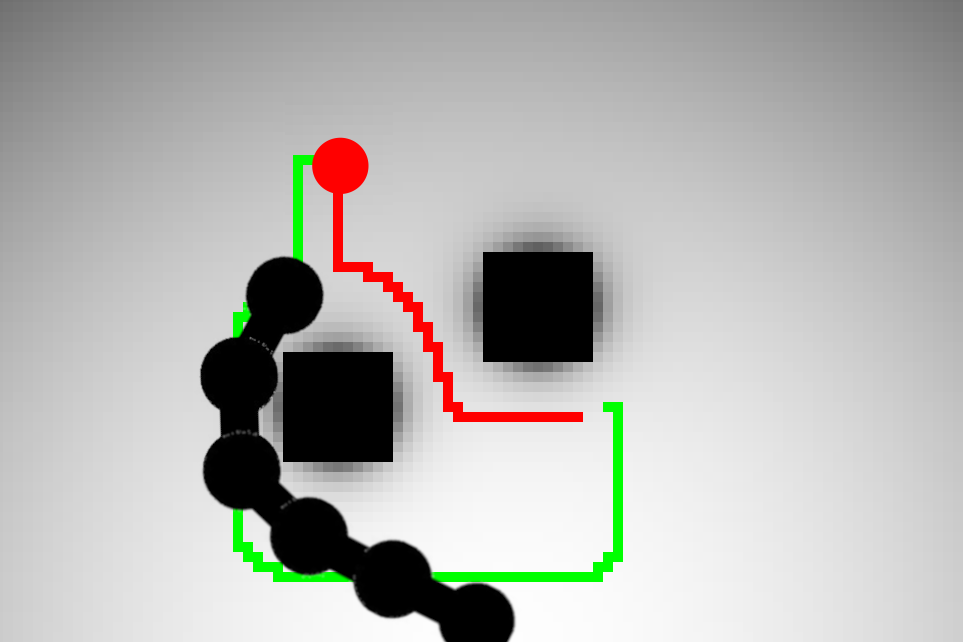
\includegraphics[width=0.99\textwidth]{manipulator_short.png}
      \caption{The careful path around obstacles does not lead to a solution, due to the manipulator being too short.}
    \end{subfigure}
    \begin{subfigure}{.3\textwidth}
      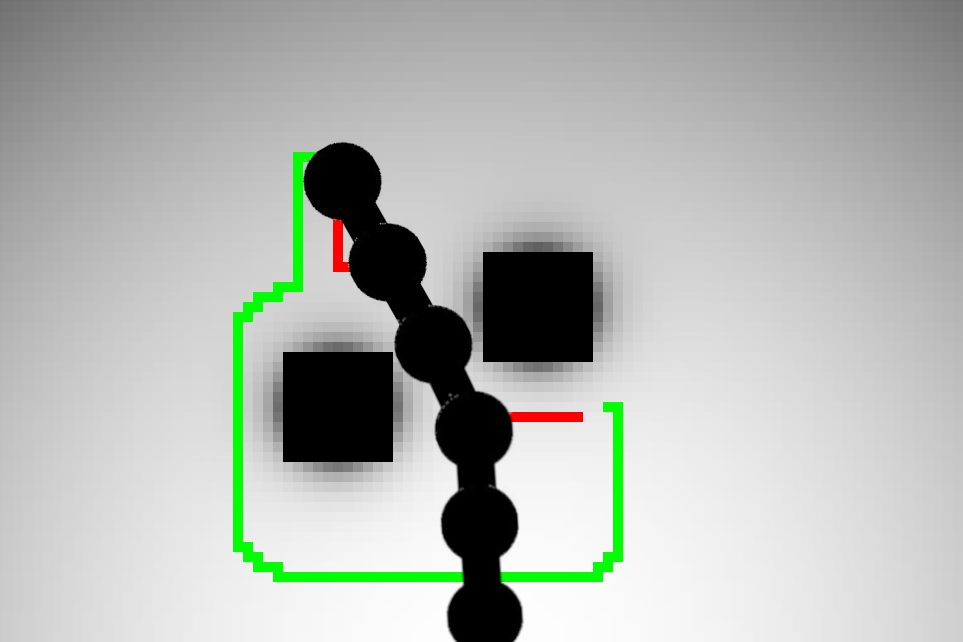
\includegraphics[width=0.99\textwidth]{manipulator_between.png}
      \caption{The viable path for the \textit{end effector} leads between the obstacles.}
    \end{subfigure}
    \caption{Illustration of the extended shortest path algorithm on a weighted grid. Black boxes represent obstacles, and the opacity of the background represents the cost of traversing over a given square.}\label{fig:paths}
\end{figure}

In effect, the algorithm works in the same fashion as APF, but does not suffer from local minima. If the first path we found is evaluated as wrong, the cost of points close to the found path is increased, and the algorithm looks for a new path in the modified graph. If, for instance, there are two obstacles and the only viable way to reach the target leads through them, paths around them may be evaluated as better at first. Trying to reproduce the path with FABRIK will fail due to the manipulator being too short, the cost near the found path is raised, and eventually the path between them is found. The idea is visualized in Figure~\ref{fig:paths}.

\begin{wrapfigure}{r}{0.4\textwidth}
  \centering
  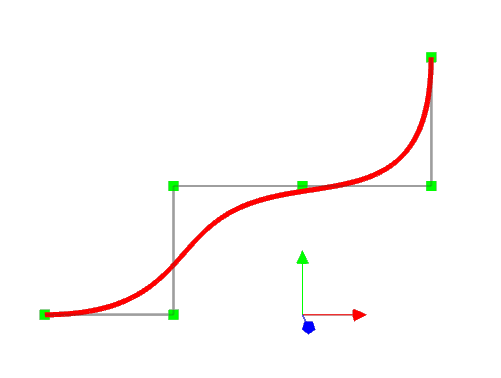
\includegraphics[width=0.4\textwidth]{nurbs_grid.png}
  \caption{B-splines can generate a smooth path from points on a grid (visualized using~\cite{nurbs_vis}).}
\end{wrapfigure}

The first obvious drawback of the algorithm is how rugged the resulting paths are. Instead of exactly following the found path and making unnecessary back and forth motion, we want to interpolate the points in a smooth way. Generating a smooth path from a set of points on the grid can be accomplished using B-splines~\cite{nurbs}.

B-splines, also known as basis splines, are piecewise polynomial functions used to generate smooth lines or shapes using a simple polynomial function and a set of control points.
To construct a B-spline, we need:

\begin{itemize}
\item A basis polynomial function given by its \textbf{order}. The order of the function determines how many nearby control points influence any the resulting points on the curve, and is always one more than the degree of the polynomial.
\item Sequence of \textbf{control points}. Control points determine the shape of the curve. Each point on the curve is determined as an interpolation between the nearby control points, using the sum of our basis functions for each of the points.
\item Sequence of \textbf{knots}. Knots are numbers in nondecreasing order, which determine where and how the control points affect the curve. The number of knots is always equal to the number of control points + the order of the curve. For trajectory generation, we can imagine the knot parameter as time. Then, we have a direct mapping of time to the position; knots specify by which control points the point will be influenced, and the ratio between the knot values specifies how much.
\end{itemize}

In the most common generalization of B-splines, Non-rational uniform B-splines (NURBS), each control point is also associated with a specific \textbf{weight}. When considering uniform points on a grid, we can just assign the same weight to each point.

Contrary to interpolating with polynomials directly, B-splines don't generally go directly through the control points. Going through a specific point can be achieved with a knot of a multiplicity equal to the order, which are commonly at the beginning and end of the curve. Since the curve order specifies how many control points influence each point, a lower curve order leads to curves closer to the control points, while a higher one can produce smoother paths overall.

\begin{figure}
  \centering
  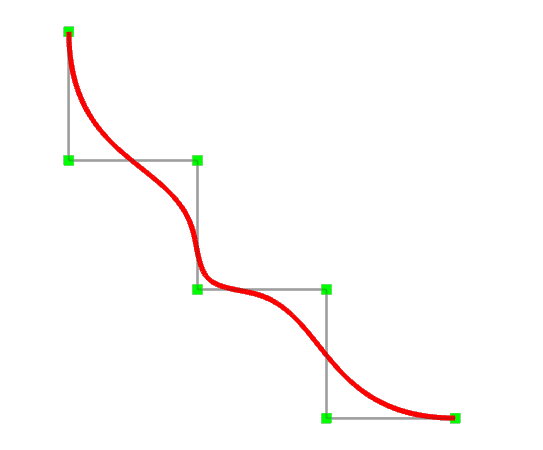
\includegraphics[width=0.5\textwidth]{nurbs_3.png}
  \caption{B-spline of order 4 with knots (0, 0, 0, 0, 0.4, 0.5, 0.6, 1, 1, 1, 1)}
\end{figure}

\begin{figure}
  \centering
  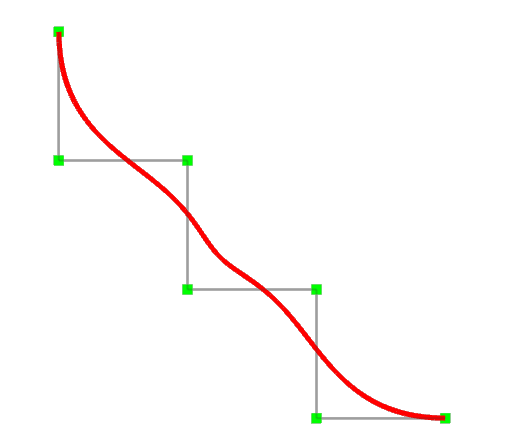
\includegraphics[width=0.5\textwidth]{nurbs_4.png}
  \caption{B-spline of order 5 with knots (0, 0, 0, 0, 0, 0.45, 0.55, 1, 1, 1, 1, 1)}
\end{figure}

To follow the curve with our inverse kinematics algorithm, we need to choose the size of our steps, get the value of the curve at the next time interval, and compute FABRIK starting at the current position. The only problem is that the curve only specifies the position, and the algorithm takes the entire transformation matrix as the input, including rotation. Hence, we need to look for ways to interpolate rotation as well.

In cases where the \textit{end effector} moves independently from the rest of the manipulator, Spherical linear interpolation (SLERP)~\cite{slerp} between the initial and target rotations is a suitable solution. The method uses quaternions to perform rotation at a constant velocity, resulting in a smooth motion.

Our case is a little different. In the case of RoFI manipulators, the rotation of the final module can influence how the entire manipulator needs to move, in order to accomodate for joint limits. Hence, we want to reach the target rotation as soon as possible. On the other hand, we need to consider that the target rotation may not be reachable immediately.

There isn't a single best way of choosing the angle interpolation, since the inputs and targets can vary wildly. A method that performs reasonably well is to interpolate euler angles of the initial \textit{end effector} position and target with a quadratic function rather than a linear one. The reasoning behind this is that early targets for FABRIK have to be close to the initial position, but the target rotation is reached quickly and we don't make unnecessary movements.

% Now that we've dealt with all the individual pieces, we have a complete algorithm.

% Let us summarize the whole process. Our input parameters are a model of the environment, which includes obstacles and a single manipulator, and a target for the manipulator.

% \begin{enumerate}
% \item The environment within which the manipulator exists is loaded, and a kinematic model of the manipulator is created.
% \item An AABB tree for collision checking is created, where the obstacles and joints are approximated via spheres.
% \item A grid is created in the space the manipulator can move in. Each obstacle raises the cost on the surrounding points of the grid.
% \item The shortest path on the weighted grid between the initial position of the \textit{end effector} and the target is found.
% \item A trajectory is created by interpolating the found path with a B-spline.
% \item The trajectory is sampled at discrete points, and an extension of FABRIK is used to compute the joint parameters needed to reach each of the points.
% \item If the path can be followed successfully, the movement is realised. Otherwise, if FABRIK fails to find viable positions on this trajectory, the algorithm falls back to step 4, adjusts the grid, and tries to find a different path.
% \end{enumerate}

% We can now demostrate initial results within a RoFI simulator. As a baseline, we will consider a manipulator that consists of a chain of 4 modules, linked via the $-Z$ connectors. Since such a manipulator has 12 degrees of freedom, previous state of the art algorithms -- which only scale up to 6 -- would clearly not be useful.

Now that we have all the pieces, we can run the algorithm and evaluate how good the paths found for the \textit{end effector} are.

Let us start by visualizing the most basic case, to see if the produced motion is natural: the algorithm in a space with no obstacles.

\begin{figure}
  \centering
  \begin{minipage}{\textwidth}
    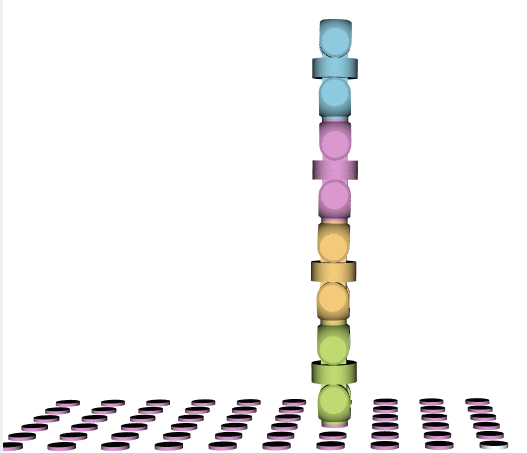
\includegraphics[width=0.3\textwidth]{sim1_0.png}
    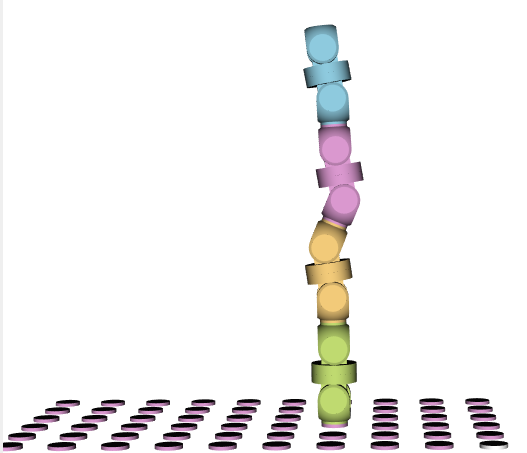
\includegraphics[width=0.3\textwidth]{sim1_1.png}
    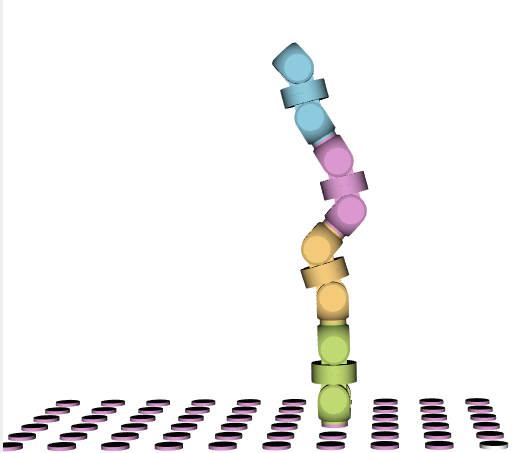
\includegraphics[width=0.3\textwidth]{sim1_2.png}

    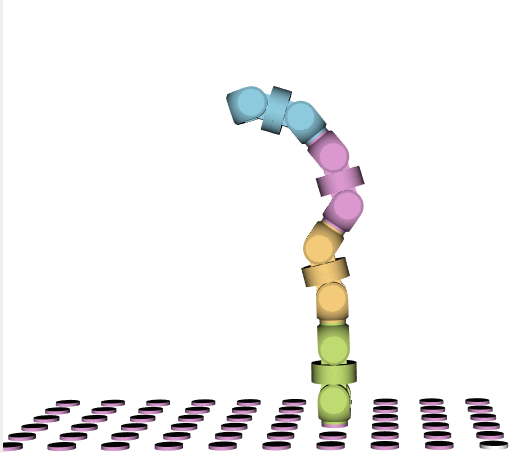
\includegraphics[width=0.3\textwidth]{sim1_3.png}
    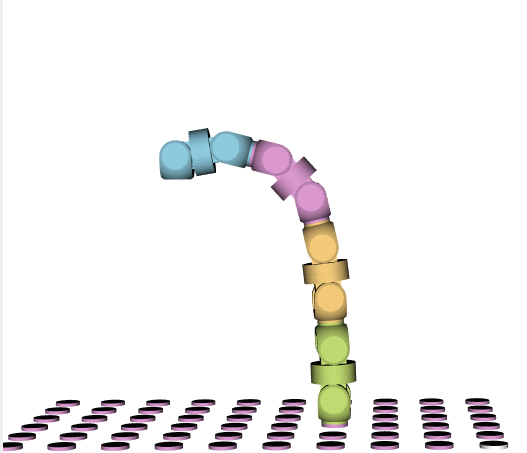
\includegraphics[width=0.3\textwidth]{sim1_4.png}
    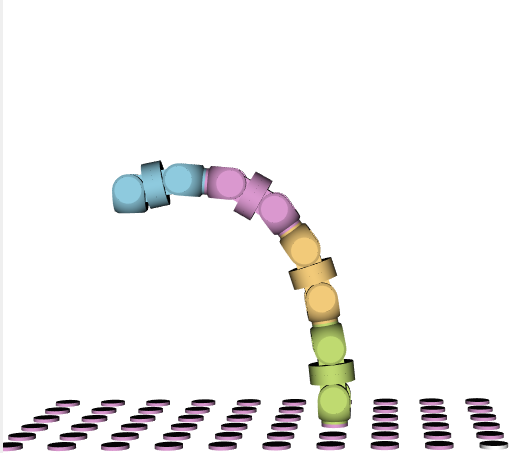
\includegraphics[width=0.3\textwidth]{sim1_5.png}
  \end{minipage}
  \caption{Our algorithm in a space with no obstacles.}\label{fig:sim1}
\end{figure}

As we can see in Figure~\ref{fig:sim1}, the found trajectory of the \textit{end effector} is smooth, including rotation. However, there is unnecessary motion before the manipulator adjusts itself into a straightened out position. Looking at the joints of the second and third module, they fold up during the algorithm, only to straighten themselves out again once the \textit{end effector} is closer to the target. We can reduce the amount of unnecessary motion by post-processing the calculated trajectory.

The post-processing algorithm is trivial: starting at the initial position, we go through the computed positions for the manipulator, and check if we can

current = initial
next = 0
while reachable (positions[next+1]):
  next += 1
current = positions[ next ]
